\subsubsection{Modulo INA}

El módulo INA es el encargado de realizar la configuración de los INAs y solicitarles medidas.
Este módulo está formado por dos archivos:
\begin{itemize}
    \item ina.cpp : Contiene las funciones necesarias para la configuración de los sensores, el bajo consumo y la toma de medidas.
    \item ina.hpp : Contiene la definición de la función que solicita 1 única medida a los INA y las direcciones I2C de los INA.
\end{itemize}

Para la implementación de este módulo se ha requerido la utilización de la librería \texttt{"INA266\_WE.h"} ,que permite configurar y leer los datos mediante I2C con Arduino.
%\TODO{ https://github.com/wollewald/INA226_WE}

El fichero ina.cpp contiene las siguientes funciones:

- \texttt{setupINA226Sensors()}: Esta función inicializa los 3 INAs con la configuración inicial que establece la librería \texttt{“INA266\_WE.h”}.

\begin{figure}[H]
    \centering
    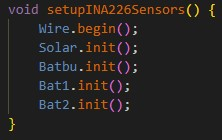
\includegraphics[width=0.5\textwidth]{images/3-software/3-2-1-ina/INA_SETUP.png}
    \caption{Configuracion Inicial INA \texttt{PS58F1}}
    \label{fig:software/INA/INA_SETUP}
\end{figure}


- \texttt{reconfig\_INAs()}: Al despertar o inicializarlos INA, se encuentran con la configuración por defecto, por lo que es necesario reconfigurarlos acorde a las necesidades de nuestro circuito. Esta reconfiguración consta de lo siguiente:
\begin{itemize}
    \item \texttt{setConversionTime}: Establece el tiempo que asignamos al INA para realizar la conversión de medidas físicas a su valor digital.
    \item \texttt{setMeasureMode}: Establece el modo de medida, POWER\_DOWN (Sistema apagado), TRIGGERED (medidas a petición) o CONTINUOUS (medidas constantes).
    \item \texttt{setResistorRange}: Establece el valor de la resistencia de SHUNT que tiene el INA (Medido físicamente) y su rango de corriente con el que se va a trabajar.
    \item \texttt{setCorrectionFactor}: Establece el factor de corrección, el sensor nunca realiza una medición que corresponde con la realidad, por lo que es necesario indicar el factor de corrección que tiene que ser aplicado cuando se realizan estas medidas. Para el establecimiento de este valor se han realizado medidas experimentales midiendo el valor real y comparándolo con lo que indicado por el sensor.
\end{itemize}

\begin{figure}[H]
    \centering
    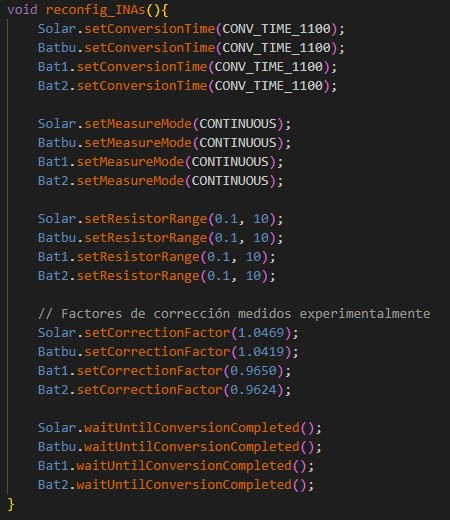
\includegraphics[width=0.5\textwidth]{images/3-software/3-2-1-ina/INA_RECONFIG.png}
    \caption{Reconfiguracion INA \texttt{PS58F1}}
    \label{fig:software/INA/INA_RECONFIG}
\end{figure}

- \texttt{powerDownINA226()}: Pone en bajo consumo los INA ya que tras conseguir las medidas no es necesario que se mantengan activos.

\begin{figure}[H]
    \centering
    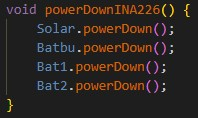
\includegraphics[width=0.5\textwidth]{images/3-software/3-2-1-ina/INA_PDOWN.png}
    \caption{INA a bajo consumo. \texttt{PS58F1}}
    \label{fig:software/INA/INA_PDOWN}
\end{figure}

- \texttt{powerUpINA226()}: Despierta de nuevo a los INA, al despertarlos los sensores se reinician con la configuración por defecto por lo que es necesario reconfigurarlos.

\begin{figure}[H]
    \centering
    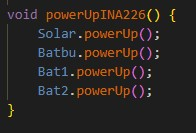
\includegraphics[width=0.5\textwidth]{images/3-software/3-2-1-ina/INA_PUP.png}
    \caption{Despertar al INA del bajo consumo. \texttt{PS58F1}}
    \label{fig:software/INA/INA_PUP}
\end{figure}


-\texttt{measureINA226(telemetry\_t *telemetry)}: Realiza la medida de todos los sensores. La secuencia de ejecución es la siguiente:

\begin{enumerate}
    \item Verifica si se han inicializado 1 vez los INAs. Si se han inicializado se despiertan.
    \item Se reconfiguran.
    \item Se toman las medidas de tensión y corriente de todos los INAs y se guarda la información en el puntero con la estructura de datos.
    \item Se ponen a bajo consumo los INAs.
\end{enumerate}

\begin{figure}[H]
    \centering
    \includegraphics[width=0.5\textwidth]{images/3-software/3-2-1-ina/INA_MEAS.png}
    \caption{Solicitar medidas al INA. \texttt{PS58F1}}
    \label{fig:software/INA/INA_MEAS}
\end{figure}


En el contenido de este mismo fichero, se instancian los 4 INAs que tenemos indicando su dirección I2C:

\begin{figure}[H]
    \centering
    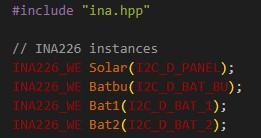
\includegraphics[width=0.5\textwidth]{images/3-software/3-2-1-ina/INA_INSTANCIA.png}
    \caption{Instancia de las direcciones de los INAs. \texttt{PS58F1}}
    \label{fig:software/INA/INA_INSTANCIA}
\end{figure}

